\documentclass[a4paper,12pt]{scrartcl}
\usepackage[utf8]{inputenc}
\usepackage[ngerman]{babel}
\usepackage[T1]{fontenc}
\usepackage{amsmath}
\usepackage{stmaryrd}
\usepackage{wasysym}
\usepackage{lmodern}
\usepackage{graphicx}
\usepackage{paralist}
\usepackage{upgreek}
\usepackage{subfigure}
\usepackage{tipa}
\usepackage{amssymb}
\usepackage{gensymb}
\usepackage{dsfont}
\usepackage{mathtools}
\usepackage{ stmaryrd }
\usepackage{fancyhdr}
\usepackage{tikz}
\usetikzlibrary{arrows,automata}

%\title{Abgabe 1}
%\author{Rafael Heid, Julian Deinert, Sabrina Buczko Gruppe\\ 6 und 7}
%\date{Abgabe am 24.10.16}

\gdef\blatt{FGI-2 Aufgabenblatt 09}

\title{\blatt}
\date{Gruppe 06}
\author{Sabrina Buczko 6663234, Julian Deinert 6535880, Rafael Heid 6704828}


\pagestyle{fancy}
\fancyhf{}
\fancyhead[L]{\blatt}
\fancyhead[R]{Buczko, Deinert, Heid}
\fancyfoot[C]{\thepage}

\begin{document}
\maketitle
\newpage
\setcounter{section}{8}
% Section 9
\section{}
\setcounter{subsection}{2}
% Section 9.3
\subsection{}
\subsubsection{}
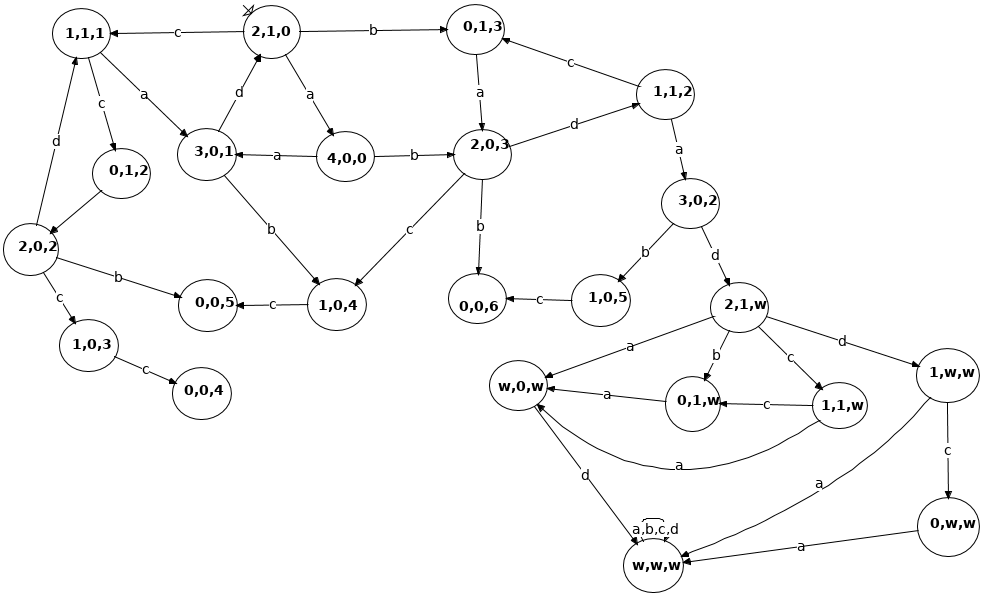
\includegraphics[scale=0.5]{netz.png}
\newpage
\subsection{}
\subsubsection{}
Die geforderte Wirkungsmatrix sieht wie folgt aus:\\\\
$
\Delta_{N_{LS}} = 
\begin{pmatrix}
-1 & 0 & 1 & -1 & 0 & 1\\
1 & -1 & 0 & 0 & 0 & 0\\
0 & 1 & -1 & 0 & 0 & 0\\
0 & 0 & 0 & 1 & -1 & 0\\
0 & 0 & 0 & 0 & 1 & -1\\
0 & -1 & 1 & 0 & -4 & 4
\end{pmatrix}
$\\\\
Durch Lösen des Gleichungssystems aus $\Delta_{N_{LS}}^{tr} \cdot i = \underline{0}$ erhalten wir die allgemeine Gleichung der P-Invariantenvektoren:\\
$
\begin{pmatrix}
p4-4 \cdot pp\\
p4-4 \cdot pp\\
p4-3 \cdot pp\\
p4-4 \cdot pp\\
p4\\
pp
\end{pmatrix}
$\\\\
Zwei explizite P-Invarianten:\\
$
\begin{pmatrix}
2\\
2\\
3\\
2\\
6\\
1
\end{pmatrix}
$
und
$
\begin{pmatrix}
1\\
1\\
3\\
1\\
9\\
2
\end{pmatrix}
$\\\\\\
Durch Lösen des Gleichungssystems aus $\Delta_{N_{LS}} \cdot j = \underline{0}$ erhalten wir die allgemeine Gleichung der T-Invariantenvektoren:\\
$
\begin{pmatrix}
p_1\\
p_1\\
p_1\\
p_2\\
p_2\\
p_2\\
\end{pmatrix}
$\\\\
Zwei explizite T-Invarianten:\\
$
\begin{pmatrix}
1\\
1\\
1\\
2\\
2\\
2
\end{pmatrix}
$
und
$
\begin{pmatrix}
2\\
2\\
2\\
3\\
3\\
3
\end{pmatrix}
$
\subsubsection{}
Die geforderte Wirkungsmatrix sieht wie folgt aus:\\\\
$
\Delta_{N_{Drohne}} = 
\begin{pmatrix}
-1 & 0 & 0 & 0 & 0 & 1\\
1 & -1 & 0 & 0 & 0 & 0\\
0 & 1 & -1 & 0 & 0 & 1\\
0 & 0 & 1 & -1 & 0 & 0\\
-1 & 0 & 0 & 0 & 0 & 1\\
0 & -1 & 0 & 0 & 1 & 0\\
0 & 0 & 0 & 1 & -1 & 0\\
0 & 0 & 0 & 0 & 1 & -1
\end{pmatrix}
$
\subsubsection{}
Menge aller S-Invariantenvektoren:\\
$\{(p_1,p_2,p_3,p_4,p_5,p_6,p_7,p_8)\ |\ p_2=p_8,\ p_3=p_4=p_7,\ p_1=p_2-p_5,\ p_6=p_3-p_2,\ p_i \in \mathbb{Z}\}$
Das Netz ist strukturell beschränkt, da eine P-Invariante in der obigen Menge ist, für die jede Stelle >0 ist.(Gezeigt in Beweis zu Theorem 7.35): (4,5,7,7,1,2,7,5)$^{tr}$, diese Invariante überdeckt ebenfalls das ganze Netz.

\subsubsection{}
\subsubsection{}
Die geforderte Wirkungsmatrix sieht wie folgt aus:\\\\
$
\Delta_{N_{DrohneNeu}} =
\begin{pmatrix}
-1 & 0 & 0 & 0 & 0 & 1 & 0\\
1 & -1 & 0 & 0 & 0 & 0 & 0\\
0 & 1 & -1 & 0 & 0 & 0 & 0\\
0 & 0 & 1 & -1 & 0 & 0 & 0\\
-1 & 0 & 0 & 0 & 0 & 0 & 1\\
0 & -1 & 0 & 0 & 1 & 0 & 0\\
0 & 0 & 0 & 1 & -1 & 0 & 0\\
\end{pmatrix}
$\\
Durch Lösen des Gleichungssystems aus $\Delta_{N_{DrohneNeu}}^{tr} \cdot i = \underline{0}$ erhalten wir die allgemeine Gleichung der P-Invariantenvektoren:\\
$
\begin{pmatrix}
0\\
0\\
p\\
p\\
0\\
p\\
p
\end{pmatrix}$\\\\
und die dazugehörige Menge:\\
$\{(0,0,p,p,0,p,p)\ |\ p \in \mathbb{Z}\}
$\\\\
Das Netz ist nicht strukturell beschränkt, da keine P-Invariante in der obigen Menge ist, für die jede Stelle >0 ist.(Gezeigt in Beweis zu Theorem 7.35)

\end{document}